\title{AI High-Performance Solution on FPGA}

\team{Nico Canzani, Dominik M\"uller}

\client{Inst. for Sensors and Electronics}

\coaches{%
  Prof. Michael Pichler,\\
  Prof. Dr. Hanspeter Schmid
}

\repo{https://git.io/aionfpga}

\fssummary{
  In a world of self-driving cars and automated quality control in manufacturing, real-time image classification is becoming increasingly important.
  Artificial intelligence (AI), and deep learning in particular, are achieving excellent classification accuracies.
  However, there are certain difficulties associated with this approach.
}

\fsgraphics{
  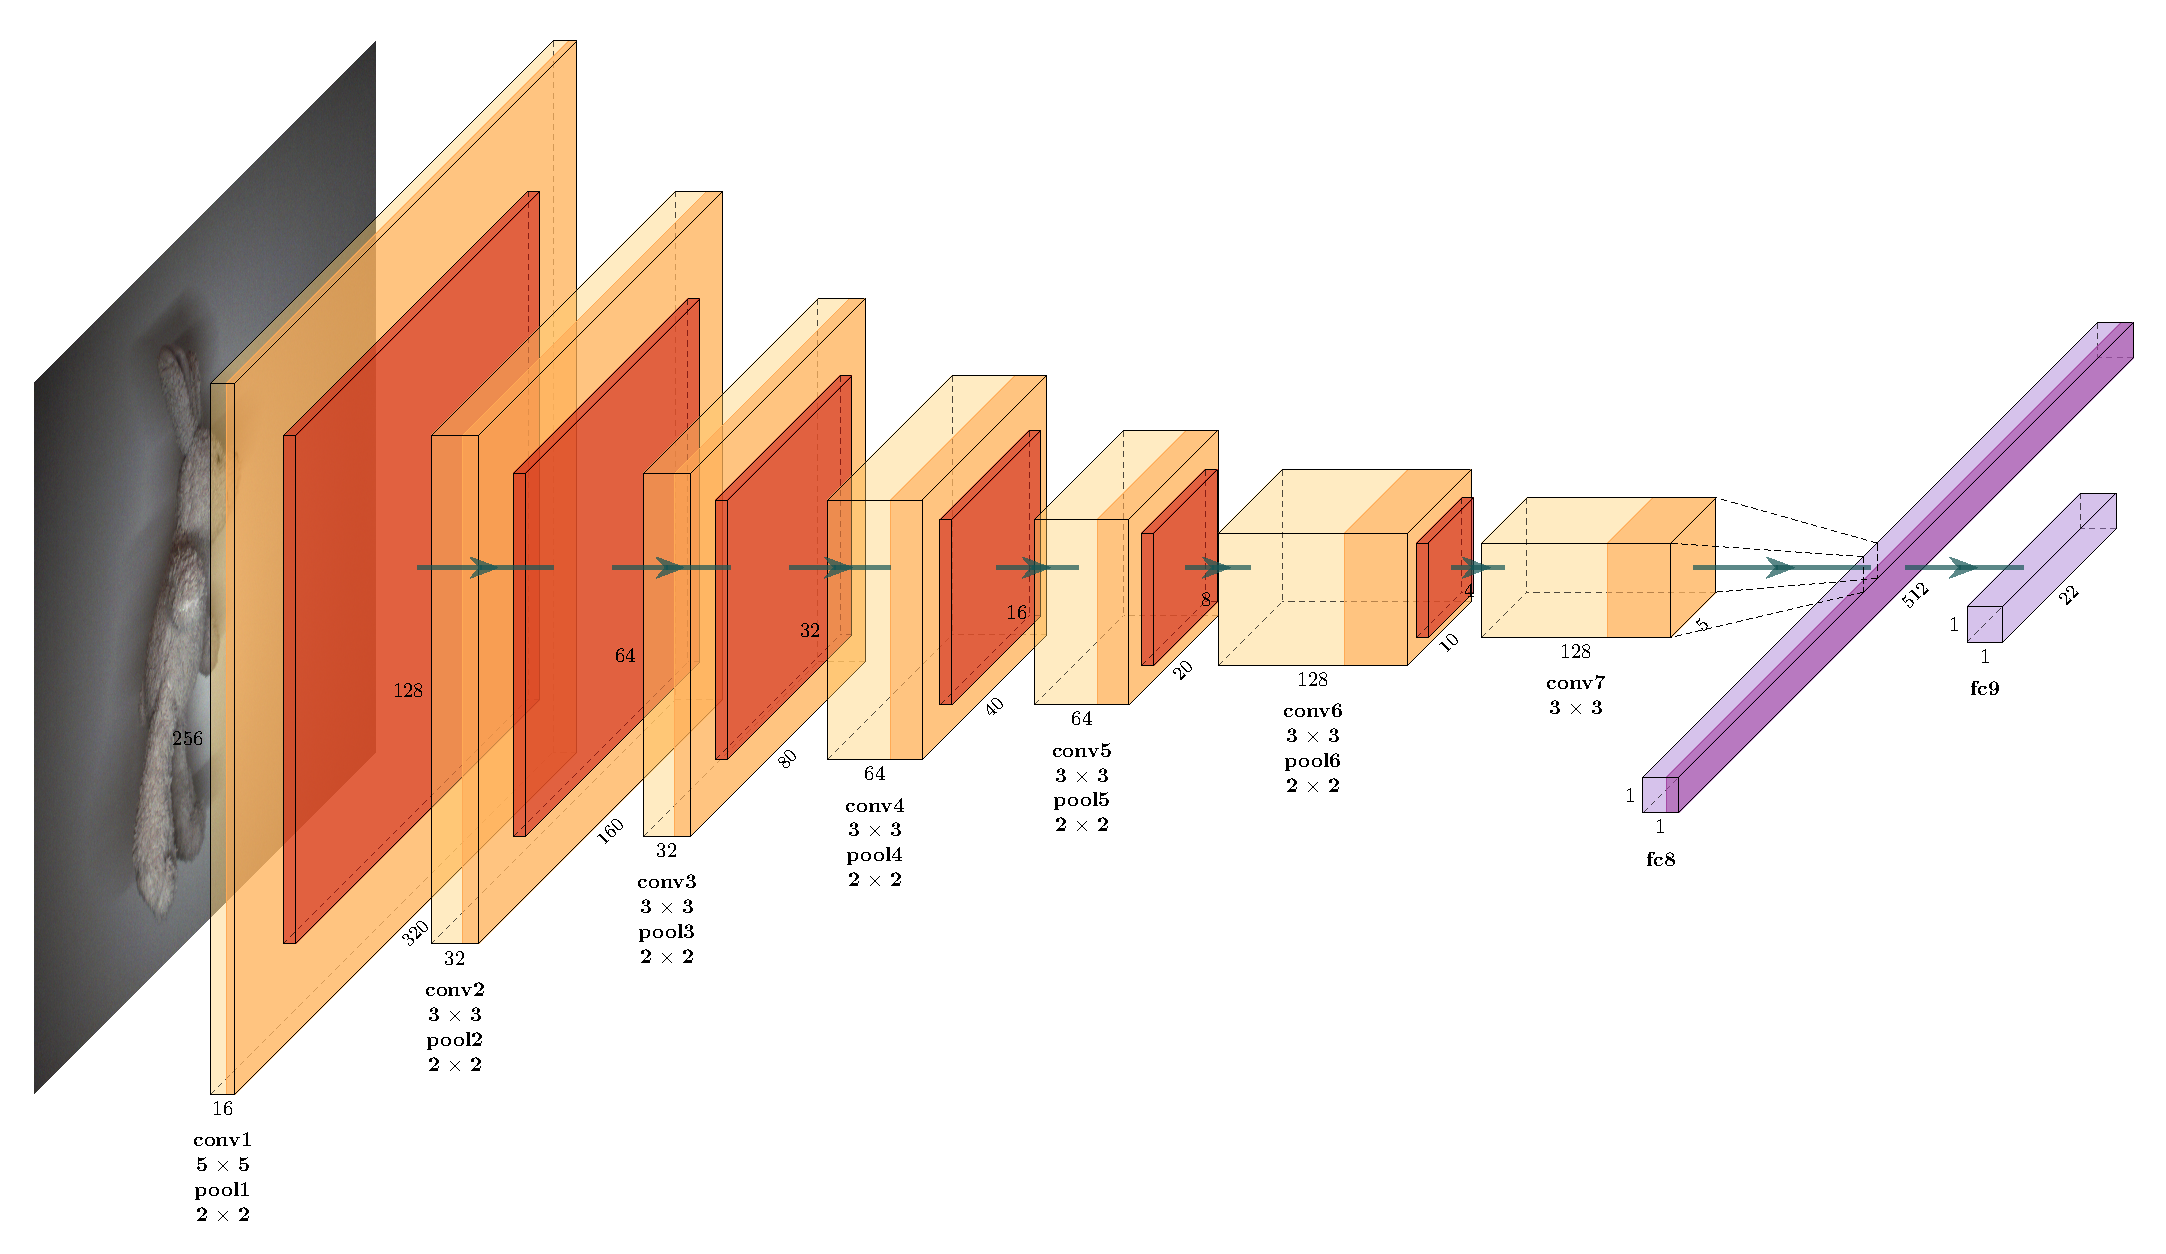
\includegraphics[width=\textwidth]{graphics/arch.pdf}
  \graphicscaption{Architecture of the Convolutional Neural Network}
}

\fscontent{
  \section{Difficulties}
  There are two main difficulties that need to be overcome.
  For one thing, high-resolution image acquisition systems require a lot of processing power.
  For another, a large labeled dataset of images is required to train deep convolutional neural networks (CNNs).
  Additionally, the training dataset must represent real-world conditions.

  \newcol
  \section{Solutions}
  A solution for the former difficulty is to use field-programmable gate arrays (FPGAs) as hardware accelerators.
  Therefore, an embedded system featuring a multiprocessor system-on-chip with an integrated FPGA is deployed.
  The second difficulty is approached with data augmentation to artificially increase the size of the labeled dataset.

  \newcol
  \section{Results}
  The result is the deep convolutional neural network shown in the image above.
  It achieves a Top-1 classification accuracy of \SI{97.2}{\percent} and a Top-5 classification accuracy of \SI{99.5}{\percent}.
  In addition, the throughput of the image classification chain reaches \SI{41.1}{fps} for color images of a size of $1280\times\SI{1024}{pixels}$.
}

\infobox{Throwing Booth}{
  \begin{minipage}{0.65\textwidth}
    The throwing booth is constructed from general-purpose aluminium profiles.
    Due to its robust impact strength, the rear panel is made of a white ABS plastic sheet and has a target hole.
    The white side panel serves as a consistent background for the images.
    It is made of a foamed PVC sheet with a fine-textured surface to reduce light reflections.
    The image acquisition system consists of a Baumer industrial camera combined with a suitable lens.
    Strong diffuse lighting is used to minimize the required exposure time and to illuminate the side panel as evenly as possible.
    Finally, a monitor is used to display the detected object.
  \end{minipage}\hfill%
  \begin{minipage}{0.32\textwidth}
    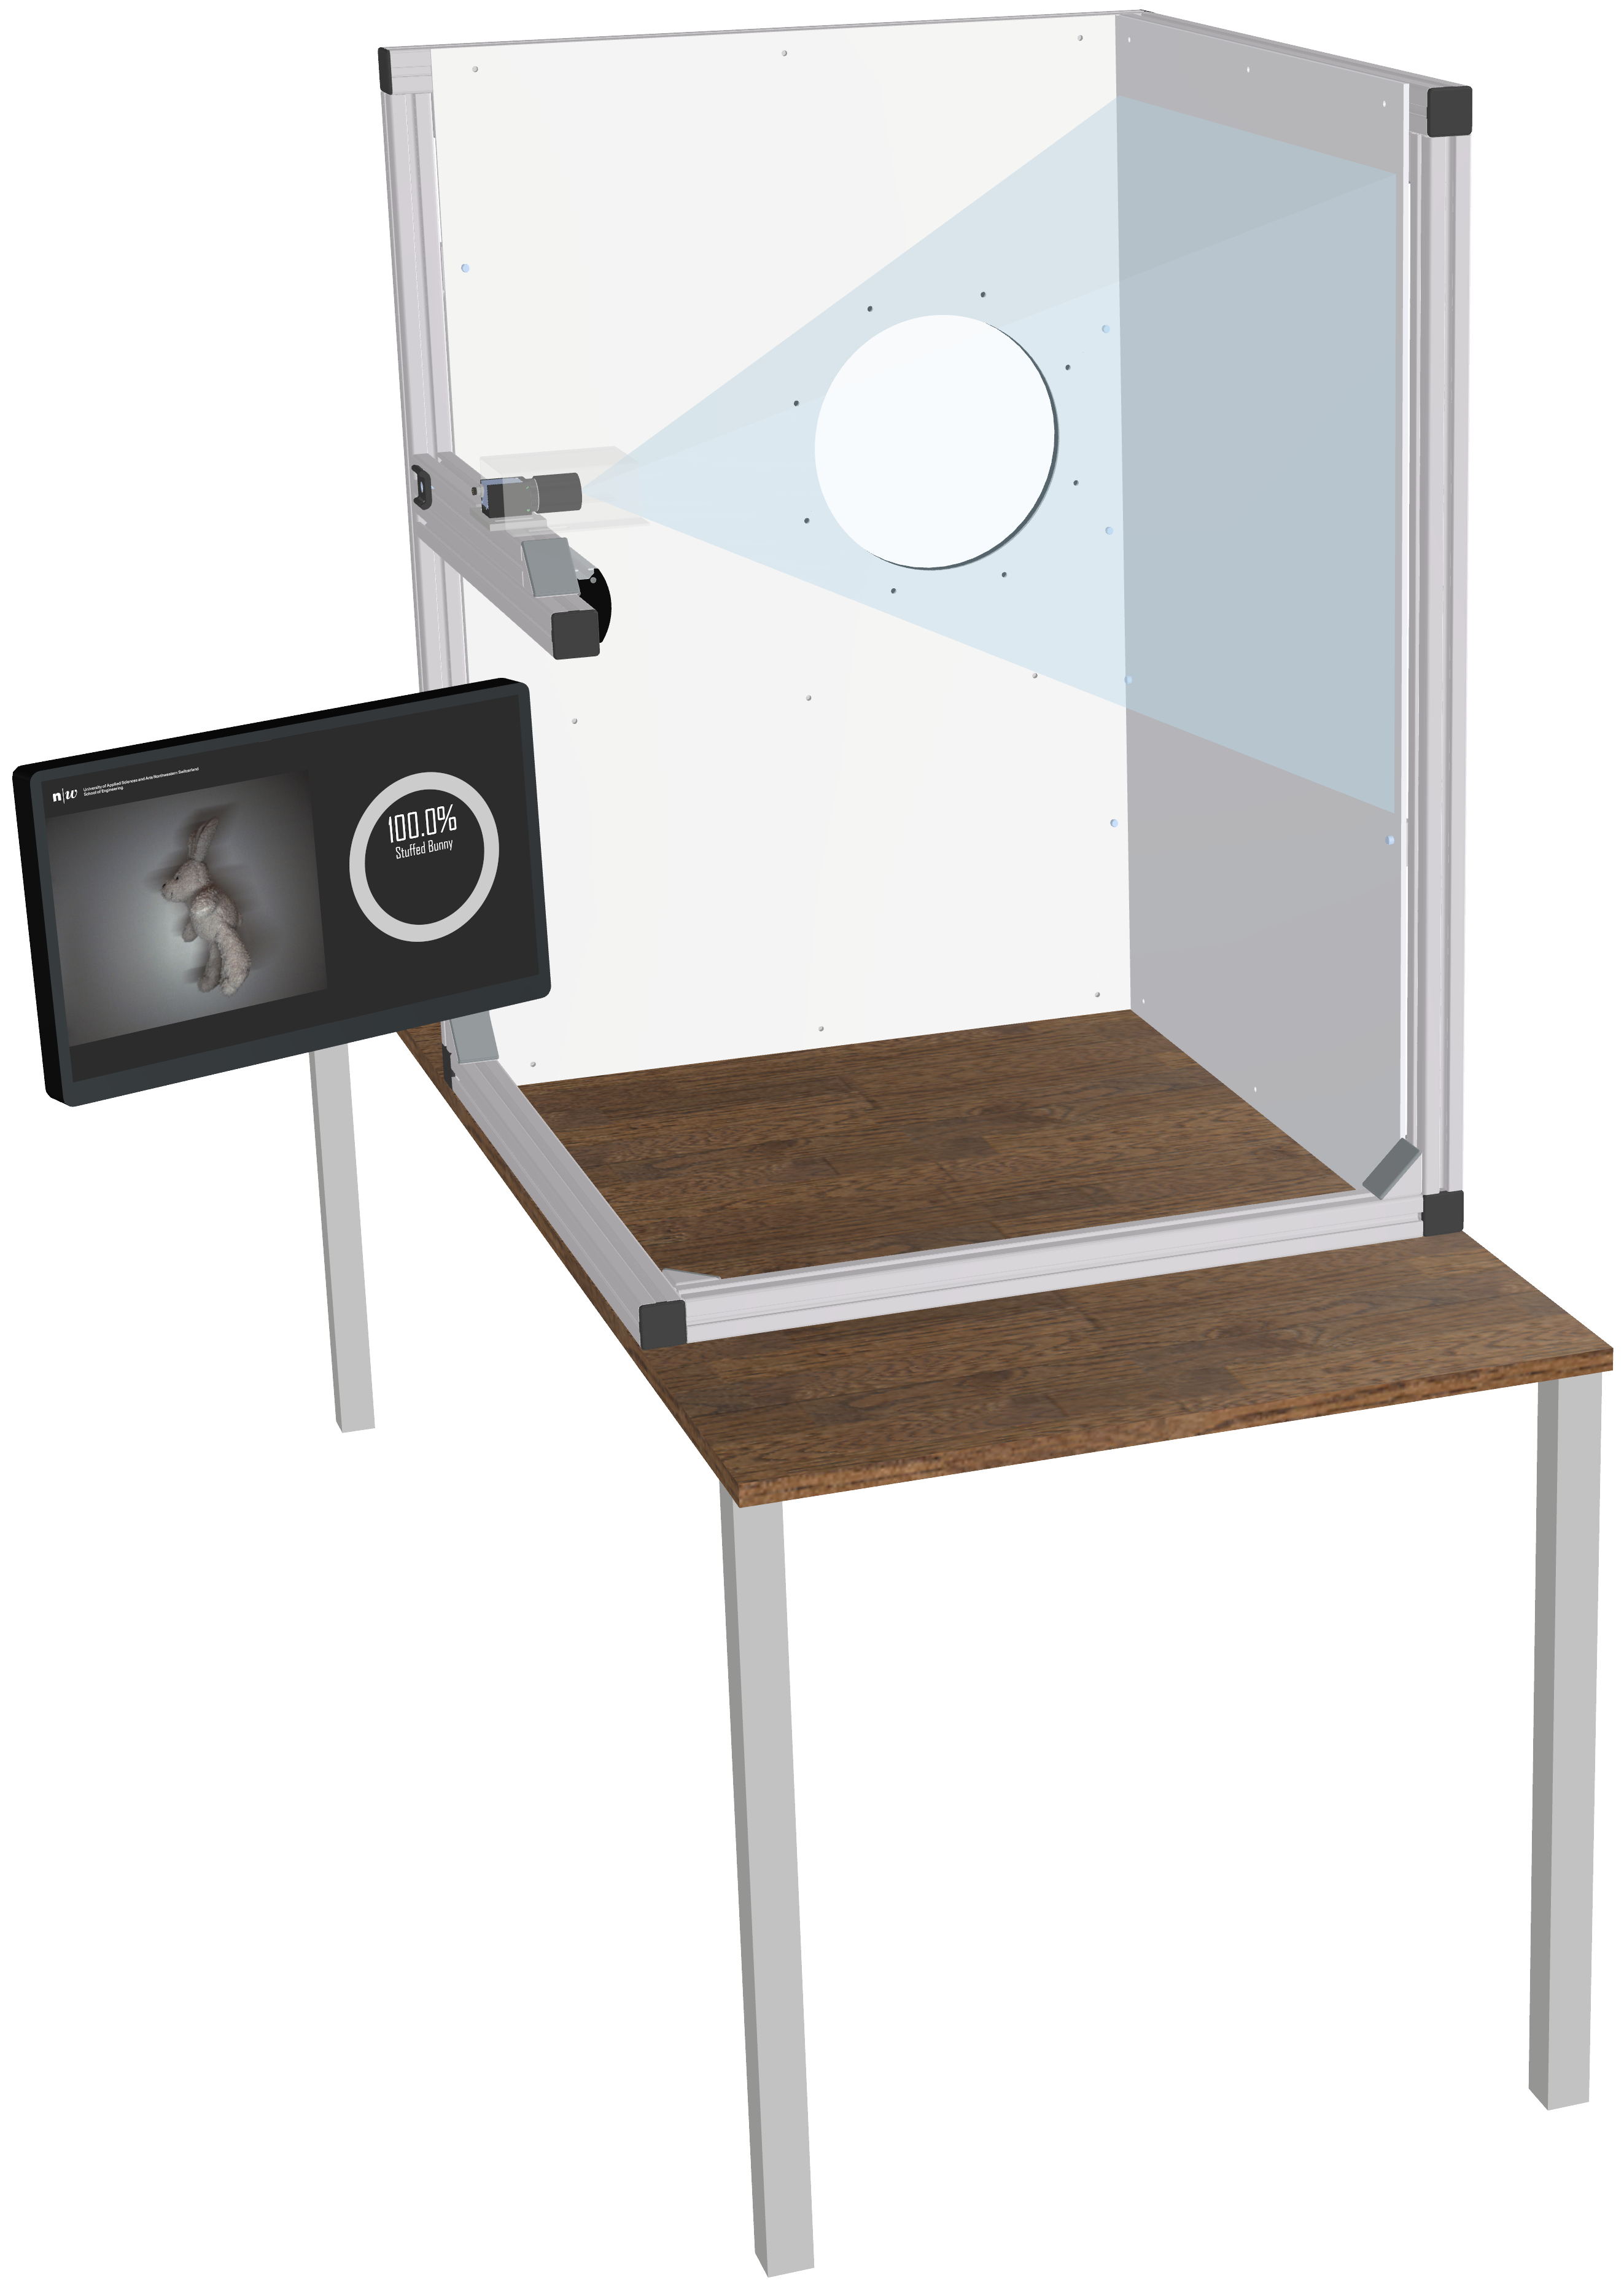
\includegraphics[width=\textwidth]{graphics/throwing_booth.png}
  \end{minipage}
}
